% !TEX TS-program = xelatex
% !TEX encoding = UTF-8 Unicode
\documentclass [ngerman,11pt]{article}
\usepackage[a4paper, top=1cm, bottom=1cm, left=2cm, right=1cm]{geometry}
\usepackage[ngerman]{babel}
\usepackage{fontspec}
\usepackage{kantlipsum}
\usepackage{enumitem}
\usepackage{xcolor}
\usepackage[many]{tcolorbox}
\usepackage{url}
\usepackage{parskip}
\usepackage{siunitx}
\sisetup{output-decimal-marker = {,}}
\newfontfamily{\FA}[Path = ./]{fontawesome-webfont}
%\def\faLink{\FA\symbol{"F0C1}}
\def\faArrow{\FA\symbol{"F0A9}\normalfont~}

\usepackage{listings}
\tcbuselibrary{listings, breakable, skins}
\lstset{ %
language=HTML,
%selectfont\ttfamily,                % choose the language of the code
basicstyle=\footnotesize,       % the size of the fonts that are used for the code
numbers=none,                   % where to put the line-numbers
%numberstyle=\footnotesize,      % the size of the fonts that are used for the line-numbers
%stepnumber=1,                   % the step between two line-numbers. If it is 1 each line will be numbered
%numbersep=5pt,                  % how far the line-numbers are from the code
%backgroundcolor=\color{white},  % choose the background color. You must add \usepackage{color}
showspaces=false,               % show spaces adding particular underscores
showstringspaces=false,         % underline spaces within strings
showtabs=false,                 % show tabs within strings adding particular underscores
frame=single,           % adds a frame around the code
tabsize=2,          % sets default tabsize to 2 spaces
captionpos=b,           % sets the caption-position to bottom
breaklines=true,        % sets automatic line breaking
breakatwhitespace=false,    % sets if automatic breaks should only happen at whitespace
escapeinside={\%*}{*)}          % if you want to add a comment within your code
}

\definecolor{shadecolor}{gray}{.85}
\pagestyle{empty}

%%%%%%%%%%%%%%%%%%%%%%%%%%%%% command definitions
\newcommand{\card}[3]{
\vfill\tcboxfit[width=18cm,height=8cm,nobeforeafter,before=\noindent,colback=white]{
\begin{tabular}{ p{0.475\linewidth} | p{0.475\linewidth}} 
\begin{minipage}[t]{\linewidth}%
{\bfseries #1}%
\par\setlength{\parskip}{6pt}%
#2%
\end{minipage}%
&
\begin{minipage}[t]{\linewidth}%
\par\setlength{\parskip}{6pt}%
#3%
\end{minipage}%
\end{tabular}
}\vfill
}

\let\oldenumerate\enumerate
\renewcommand{\enumerate}{
\oldenumerate[wide, labelwidth=!, labelindent=0pt]
}

\let\olditemize\itemize
\renewcommand{\itemize}{
\olditemize[wide, labelwidth=!, labelindent=0pt]
}


%%%%%%%%%%%%%%%%%%%%%%%%%%%%% document
\begin{document}

\begin{center}
{\bfseries\sffamily \Large\bf Lernkarten A-FRAME}\\[2mm]
von Till Zoppke

\end{center}
\hrule
\medskip

Die Lernkarten wurden erstellt für den Ferienkurs ``ProInformatik V'', 6.-10. August 2018, an der Freien Universität Berlin.

Die Karten sind nach Themen gegliedert. Zu den Karten gibt es auch einen Spielplan, auf dem die Lernenden ihren Fortschritt mit einer Spielfigur markieren können.

Jede Lernkarte bietet eine oder mehrere Aufgaben zur Lernkontrolle und Raum für Notizen. Die Lernenden sammeln die Lernkarten in einem Hefter und haben so Unterlagen aus dem Kurs. So wie Kontoauszüge symbolisieren die Karten den Lernfortschritt der Lernenden. Mit jeder bearbeiteten Lernkarte zahlen sie auf ihr Wissenskonto ein.

Zu den Lernkarten gibt es eine Website. Diese enthält die auf den Lernkarten angegebenen Links, so dass die Lernenden diese nicht abtippen müssen.

Auf der Checkliste sind alle Lernkarten verzeichnet. Die Lernenden können abhaken, wenn sie eine Karte erledigt haben. Ihr Ergebnis sollen Sie dem Kursleiter, dem Tutor oder einem anderen Lernenden zeigen, der dann abzeichnet, dass die Aufgabe gelöst wurde (Vier-Augen-Prinzip).

{\bfseries\large Legende}\\
\begin{itemize}
\item Die auf einer Lernkarte definierten oder erläuterten Begriffe sind {\bfseries fett} markiert.
\item Wenn auf Begriffe von anderen Lernkarten verwiesen wird, so sind diese \underline{unterstrichen}.
\item Quelltext und Tastaturküzel sind in \texttt{Monospaced} gesetzt.
\item Links zu Web-Ressourcen, die von der Kursseite aus zugänglich sind, sind mit einem \faArrow\normalfont~Pfeil markiert.
\end{itemize}

\vfill

\includegraphics[width=2cm]{CC-BY-SA}
\pagebreak

%%%%%%%%%%%%%%%%%%%%%%%%%%%%% cards

%%% Abschnitt 1: Werkzeuge

\card{Werkzeuge: Firefox}{ %%%
Wir entwickeln ein Internet-Projekt. Oder genauer: eine Website im World-Wide-Web, auf der VR-Inhalte dargestellt werden. Seit der Erfindung des World-Wide-Web hat sich der Web-Browser als Programm zur Darstellung von Websites herausgebildet. Er kann den Seitenquelltext interpretieren und die Seite für den Nutzer darstellen. Für unser Projekt nutzen wir den Webbrowser Firefox. 
\begin{enumerate}
\item Recherchieren Sie im Internet, welche Eigenschaften der Firefox gegenüber anderen Browsern hat, die für unser Projekt vorteilhaft sein könnten.
\item Argumentieren Sie, welchen Sinn es macht, dass wir uns im Projekt auf einen Standard-Browser einigen.
\end{enumerate}
{}}

\card{Werkzeuge: git \& github}{ %%%
Sie kennen es von Ihrem Handy: ständig kommen neue Versionen des Betriebssystems und von Apps mit Verbesserungen oder Bugfixes heraus. Das alles muss programmiert werden. Für die Verwaltung des Programmcodes nutzen Softwareentwickler ein Werkzeug vom Typ {\bfseries Versionsverwaltung}. Diese führt über alle Änderungen Buch und ermöglicht es, Patches zu generieren und auf ältere Versionen einer Datei zurückzugreifen.\par
Die zur Zeit populärste Webplattform für Softwareprojekte namens {\bfseries github} basiert auf der Versionsverwaltung {\bfseries git}. In diesem Projekt werden wir auf eine Versionsverwaltung verzichten, um die Einarbeitungszeit zu sparen. Wir benötigen jedoch einen github-Account, um den Online-Editor {\bfseries glitch} benutzen zu können.}
{\begin{enumerate}
\item Öffnen Sie \faArrow \url{https://github.com} im Browser und registrieren Sie sich für einen Account.
\item Schauen Sie nach, an welchen Projekten Ihr Kursleiter in den letzten beiden Wochen gearbeitet hat.
\end{enumerate}}

\card{Werkzeuge: glitch}{ %%%
Auf der Plattform {\bfseries glitch} lassen sich Web-Projekte entwickeln und teilen. Der {\bfseries Online-Editor} mit Syntax-Highlighting für gängige Programmier- und Auszeichnungssprachen (HTML, JavaScript, CSS$\ldots$) ermöglicht mehreren Leuten kollaborative Zusammenarbeit an der gleichen Datei. Mit der Funktion ``Live'' wird das Projekt auf einem Server gestartet und kann getestet werden.
\begin{enumerate}
\item Loggen Sie sich mit Ihrem github-Account auf \newline\faArrow \url{https://glitch.com} ein.
\item Öffnen Sie unter \url{https://glitch.com/@accountname} Ihre Nutzereinstellungen und laden Sie ein Avatarbild hoch. Anhand des Avatarbilds kann man erkennen, wer an welchen Projekten arbeitet.
\end{enumerate}
\vspace{0cm}
}{\begin{enumerate}\setcounter{enumi}{3}
\item Öffnen Sie den Quelltext der Informationsseite zu unserem Kurs (den Link erhalten Sie per Email). 
\item Schreiben Sie zwischen die beiden grauen Kommentare ein kleines Statement (z.B. \emph{Hallo Welt!}) zum Kurs.
\item Testen Sie Ihre Änderungen, indem Sie die Schaltfläche ``Live'' betätigen und das Aussehen der veränderten Seite überprüfen.
\end{enumerate}}

\card{Werkzeuge: Tastaturkürzel}{ %%%
Für häufig genutzte Funktionen gibt es auch in \underline{glitch} {\bfseries Tastaturkürzel}. Vorteil von Tastaturkürzeln ist, dass man beim Arbeiten Zeit spart. Nachteil ist, dass man die Kürzel auswendig lernen muss. Man muss also einmal zu Beginn Zeit investieren, um die Kürzel zu lernen, die sich über einen längeren Zeitraum hinweg wieder auszahlt. Daraus folgt: je eher man Tastaturkürzel lernt, desto größere Zeitersparnis bieten sie.
\begin{enumerate}
\item Öffnen Sie ein glitch-Projekt Ihrer Wahl und testen Sie die angegebenen Tastaturkürzel im Editor aus.
\item Wählen Sie im Editor die Funktion ``Glitch-Options'' $\rightarrow$ ``Keyboard Shortcuts''. Probieren Sie die Funktionen aus, die Ihnen interessant erscheinen.
\item Öffnen Sie die \faArrow Übersicht der Sublime-Tastaturkürzel. Die meisten sind auch in glitch verwendbar, probieren Sie einige aus.
\end{enumerate}}
{\begin{itemize}
\item Mit \texttt{Shift + Cursortasten} lässt sich Text markieren, ohne die Maus zu benutzen.
\item Markieren Sie einige Zeilen und drücken Sie \texttt{Tab}, um den Text einzurücken.
\item Mit \texttt{Shift + Tab} können Sie die Einrückung wieder verringern.
\item Mit \texttt{Ctrl + Shift + K} löschen Sie die aktuelle Zeile.
\item Mit \texttt{Ctrl + /} können Sie Programmcode \underline{auskommentieren}, um ihn für den Interpreter unsichtbar zu machen.
\item Sie machen die letzten Änderungen Schritt für Schritt rückgängig, indem Sie \texttt{Ctrl + z} betätigen.
\item Mit \texttt{Ctrl + Shift + Z} werden die Änderungen wiederhergestellt.
\end{itemize}
}

%% Abschnitt 2: Grundlagen

\card{Grundlagen: HTML}{ %%%
Mit der Auszeichnungssprache {\bfseries HTML} werden Webseiten gestaltet. In HTML wird natürliche Sprache mit sogenannten Tags strukturiert. Ein {\bfseries Tag} wird mit spitzen Klammern notiert. Bis auf wenige Ausnahmen gibt es zu jedem ``öffnenden'' Tag auch einen ``schließenden''. In dem folgenden Beispiel wird eine Überschrift (engl.: Heading) der Ebene 2 kodiert:
\par
\texttt{<h2>\newline
~~Das letzte Wort ist\newline
~~<font color="\#0000FF">blau</font>\newline
</h2>}
\par
Das Framework \underline{A-FRAME}, das wir für unser VR-Projekt verwenden, setzt auf HTML auf. Sie brauchen nicht alle HTML-Tags zu kennen, wohl aber die Syntax und das {\bfseries HTML-Grundgerüst}.
}{\begin{enumerate}
\item Falls Sie mit HTML noch nicht vertraut sind, lesen Sie \faArrow Kapitel 1 des HTML-Tutorials ``Grundgerüst einer HTML-Seite''.
\item Öffnen Sie die \faArrow einfache Website und überprüfen Sie anhand Ihres Avatars, dass Sie bei glitch angemeldet sind.
\item Gehen Sie auf die Projekt-Optionen und erstellen Sie einen Remix. Sie haben nun eine Kopie der Seite erzeugt, die Ihrem Account zugeordnet ist und die Sie beliebig verändern können.
\item Fügen Sie einige neue Elemente zur Website hinzu.
\end{enumerate}
}

\card{Grundlagen: Hexadezimalsystem}{ %%%
Wahrscheinlich haben Sie schon davon gehört, dass Zahlen im Computer mit Nullen und Einsen dargestellt werden. Die binäre Ziffernfolge $(1101)_2$ beispielsweise entspricht der Zahl $(11)_{10}$ im Dezimalsystem. Man rechnet so: $1\cdot2^0 + 0\cdot2^1+1\cdot2^2+1\cdot2^3 = 11$.
\par
Um Platz zu sparen, kann man vier solcher Binärziffern zusammenfassen und im sogenannten {\bfseries Hexadezimalsystem} darstellen. Mit vier Binärziffern lassen sich Zahlenwerte zwischen $(0000)_2=(0)_{10}$ und $(1111)_2=(16)_{10}$ darstellen. Für Zahlen im Hexadezimalsystem braucht man also insgesamt 16 Ziffern. Man nimmt hierfür die bekannten Ziffern 0-9 aus dem Dezimalsystem und zusätzlich noch die Buchstaben A-F, und weist diesen die Werte $(A)_{16}=(10)_{10}$ bis $(F)_{16}=(15)_{16}$ zu.}
{\begin{enumerate}
\item Falls Sie gerade zum ersten mal Hexadezimalzahlen gesehen haben, lassen Sie sich es noch mal vom Kursleiter oder Tutor erklären. Für A-Frame brauchen wir keine Zahlen umrechnen, aber z.B. Farbwerte werden hexadezimal dargestellt.
\item Rechnen Sie die folgenden Zahlen ins Dezimal- bzw. Hexadezimalsystem um.
\begin{enumerate}
\item $(77)_{16}=$
\item $(A1)_{16}=$
\item $(100)_{10}=$
\item $(128)_{10}=$
\end{enumerate}
\item Spielen Sie eine Runde \faArrow Binary Blitz und notieren Sie Ihren Highscore.
\end{enumerate}}

\card{Grundlagen: Syntax}{ %%%
Als {\bfseries Syntax} einer Sprache bezeichnet man eine Menge von Regeln, nach denen Ausdrücke in dieser Sprache gebildet werden. Für natürliche Sprachen sind dies Grammatik, Zeichensetzung und Rechtschreibung.
\par
Ob ein Ausdruck syntaktisch korrekt ist, kann man gut mit einem Algorithmus überprüfen. Bei unserem Projekt unterstützt uns \underline{glitch} und markiert alle Syntax-Fehler, die wir in \underline{HTML} oder \underline{JavaScript} machen, mit einem roten Punkt. 
\par
Glitch hebt außerdem die Syntax von HTML und JavaScript hervor, indem es Elemente farbig markiert. HTML-Tags z.B. werden blau gefärbt, Zeichenketten braun und \underline{Kommentare} grau.
}{
\begin{enumerate}
\item Öffnen Sie das glitch-Projekt \faArrow Syntaxfehler und erstellen Sie einen Remix. Finden und korrigieren Sie dann die Syntaxfehler. Typische Fehler sind:
\begin{itemize}
\item schließender Tag vergessen
\item Tags werden in falscher Reihenfolge geschlossen
\item HTML-Grundgerüst nicht beachtet
\item Anführungszeichen vergessen
\item Dezimalbrüche mit Komma statt mit Punkt (Im Angelsächsischen Raum werden bei Fließkommazahlen (Engl. Foating-Point-Numbers) die Nachkommastellen mit einem Punkt abgetrennt)
\end{itemize}
Tipp: Gehen Sie bei der Fehlersuche von oben nach unten vor.
\end{enumerate}}

\card{Grundlagen: Lebarkeit}{ %%%
Das Wichtigste bei einem Programm ist seine Korrektheit, also dass es das tut, was es tun soll. Ein weiterer Qualitätsaspekt ist die {\bfseries Lesbarkeit}, die man durch {\bfseries Einrücken} des Quelltextes erhöhen kann. 
\begin{itemize}
\item Wenn ein öffnender Tag in der selben Zeile wieder geschlossen wird, geht es in der nächsten mit der gleichen Einrückung weiter.
\item Ansonsten wird nach einem öffnenden Tag die nächste Zeile um zwei Leerzeichen weiter nach rechts eingerückt.
\item Nach einem schließenden Tag verringert sich die Einrückung um zwei Leerzeichen.
\end{itemize}}
{Die Lesbarkeit erhöht sich außerdem durch das Einfügen von {\bfseries Kommentaren}. Kommentare sind Texte von Menschen für Menschen, die vom Computer ignoriert werden, und die Funktionen des Programmcodes in natürlicher Sprache erläutern.\newline
\texttt{<!-- Dies ist ein Kommentar in HTML -->}
\begin{enumerate}
\item Öffnen Sie die \faArrow Seite zum Einrücken. Der Seitenquelltext ist mit der einfachen Website, von der Sie einen Remix erstellt haben, identisch, nur sind einige Zeilen anders umgebrochen und Einrückungen sind falsch.
\item Rücken Sie die Zeilen gemäß den links angegebenen Regeln ein. Vergleichen Sie Ihr Ergebnis mit der einfachen Website.
\item Fügen Sie auch einen Kommentar ein.
\end{enumerate}}

%% Abschnitt 3: A-FRAME

\card{A-FRAME: Geometrische Körper}{ %%%
Die einfachsten Objekte, die sich in A-FRAME darstellen lassen, sind {\bfseries geometrische Körper}. Hierzu schauen wir uns eine einfache Szene an, die von A-FRAME zum Einstieg bereitgestellt wird.
\begin{enumerate}
\item Öffnen Sie die Seite \faArrow Hello WebVR und klicken Sie auf ``View Source''. Wählen Sie dann links in der Sitebar ``index.html''.
\item Lesen Sie die Erläuterungen (rechts) zu der Seite.
\item Erstellen Sie einen Remix und verändern Sie die Größe der Objekte.
\end{enumerate}}
{\begin{itemize}
\item Das Grundgerüst der Seite ist das gleiche wie für alle HTML-Webseiten. Um die Funktionen von A-FRAME verfügbar zu machen, wird in Z.7 die A-FRAME-Bibliothek eingebunden.
\item Die von A-FRAME zur Verfügung gestellten Tags haben alle die Form \texttt{<a-tagname>}.
\item Mit \texttt{<a-scene>...</a-scene>} wird der Bereich für unsere VR-Welt definiert. Mit dem Attribut \texttt{background} wird eine \underline{Hintergrundfarbe} für die Szene definiert.
\item Die Szene enthält vier Elemente: Einen Quader (box), eine Kugel (sphere), einen Zylinder und eine Ebene (plane).
\item Die Größe der Objekte ist durch die Attribute \texttt{radius}, \texttt{width} und \texttt{height} gegeben.
\end{itemize}
}

\card{A-FRAME: 3D-Koordinaten}{ %%%
Zu den beiden Dimensionen, die Sie als X- und Y-Achse von der Tafel aus dem Mathematikunterricht kennen, kommt in VR-Welten noch eine {\bfseries 3. Dimension} hinzu, die Z-Achse. Das Koordinatensystem in A-Frame ist {\bfseries rechtshändig}. Das bedeutet, die Achsen sind so im Raum orientiert, wie in der Skizze rechts angegeben.
\par
Sofern es nicht anders definiert ist, startet die Kamera im Ursprung $(0,0,0)$ des Koordinatensystems und blickt in den Halbraum mit negativen Z-Werten (also in die entgegengesetzte Richtung, als die der Mittelfinger zeigt).
\begin{enumerate}
\item Verändern Sie in Ihrem Remix von \faArrow Hallo WebVR die Koordinaten der Objekte und beobachten Sie, was passiert.
\end{enumerate}}
{\begin{center}
{\bfseries Rechte-Hand-Regel}\par\vspace{0.5cm}
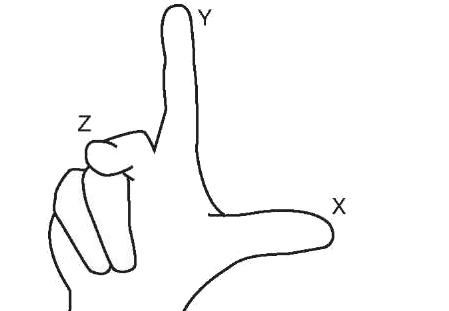
\includegraphics[width=6cm, trim= 0 0 1cm 0, clip=true]{handregel}
\end{center}}

\card{A-FRAME: Drehung im Raum}{ %%%
Objekte können im Raum gedreht werden. Hierzu gibt man für jede {\bfseries Drehachse} an, um wieviel Grad der Körper um sie gedreht werden soll. Hierbei wird zunächst um die X-Achse, dann um die Y-Achse und schließlich um die Z-Achse gedreht. {\bfseries Drehpunkt} ist der Mittelpunkt des Körpers.
\begin{enumerate}
\item Nehmen Sie einen Gegenstand (z.B. Ihr Handy) und drehen Sie ihn aus seiner Ursprungsposition jeweils
\begin{enumerate}
\item 90 Grad um die X-Achse 
\item -90 Grad um die Y-Achse
\item 45 Grad um die Z-Achse
\end{enumerate}
\item Verändern Sie in Ihrem Remix von \faArrow Hallo WebVR die Rotation der Objekte und beobachten Sie, was passiert.
\end{enumerate}}
{\begin{center}
{\bfseries Korkenzieherregel}\par\vspace{0.4cm}

\includegraphics[width=5cm]{korkenzieherregel}
\end{center}
Die Drehrichtung kann man sich nach der Korkenzieherregel veranschaulichen.}

\card{A-FRAME: Farbe}{


%\card{A-FRAME: Slack-Channel}{ %%%
%\card{A-FRAME: Camera}{ %%%
%\card{A-FRAME: Zusammengesetzte Objekte}{ %%%

%\card{Grundlagen: Java-Script}{ %%%

\end{document}
